\begin{frame}
	\frametitle{Github}
	\framesubtitle{Init a repository}
	\addtocounter{nframe}{1}
	
		\begin{block}{Github platform}
		GitHub is the largest host for git repositories. It is a central point of collaboration among developers.
 		\end{block}

		 \begin{block}{Github capabilities}
			Git hosting, issue tracking, code review, and other things
		\end{block}
	
\end{frame}
	
\begin{frame}
\frametitle{Github}
\framesubtitle{Init a repository}
\addtocounter{nframe}{1}

	\begin{center}
		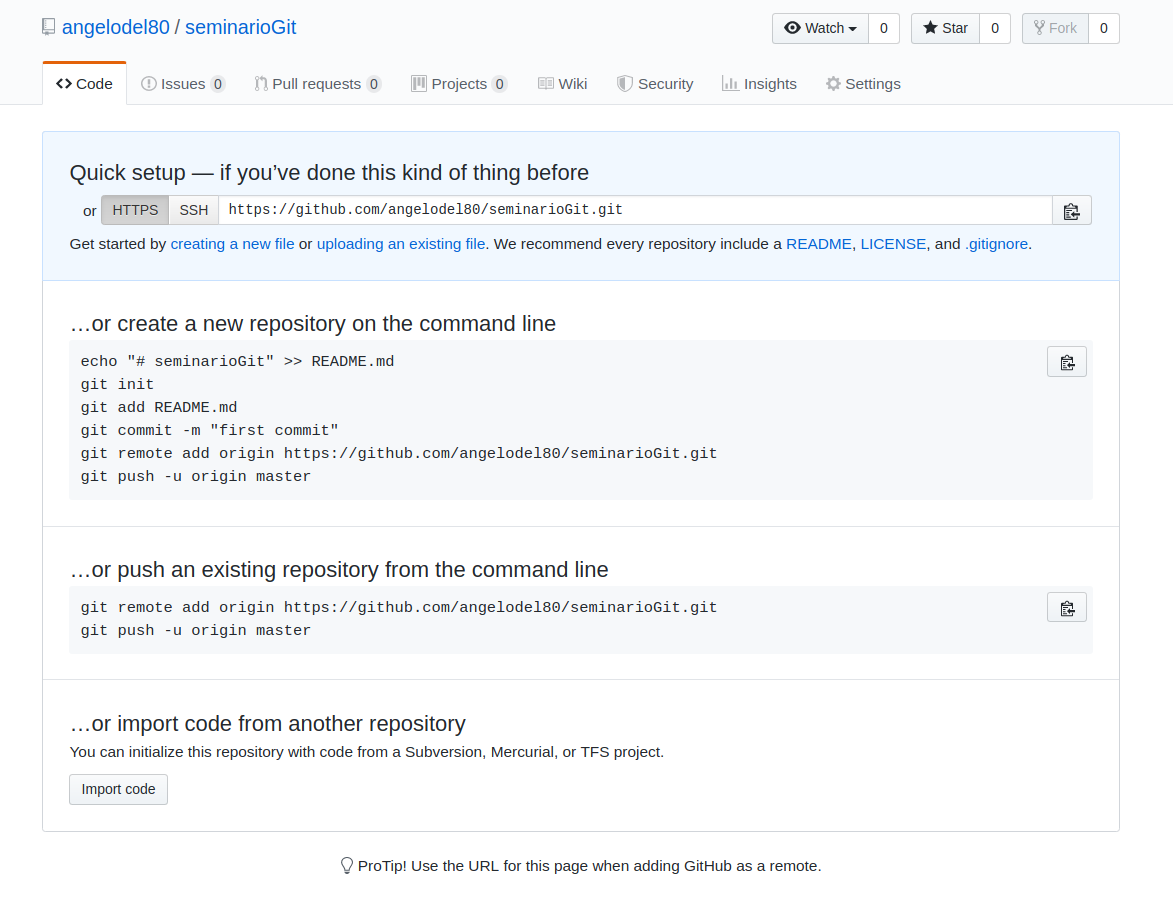
\includegraphics[width=.9\textwidth]{imgs/GitHub-RepoInit.png}
	\end{center}

\end{frame}

\begin{frame}
	\frametitle{Github}
	\framesubtitle{adding collaborators}
	\addtocounter{nframe}{1}
	
	
		\begin{center}
			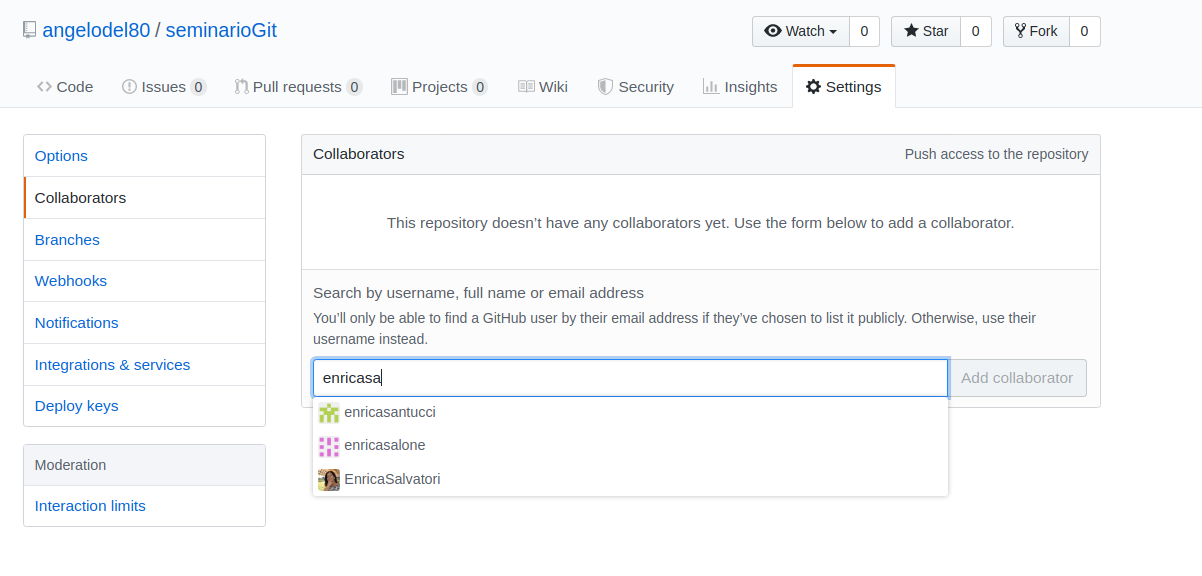
\includegraphics[width=.95\textwidth]{imgs/github-Collaborators.png}
		\end{center}
	
\end{frame}

\begin{frame}
		\frametitle{Github}
		\framesubtitle{Comments to content lines}
		\addtocounter{nframe}{1}
		
			\begin{center}
				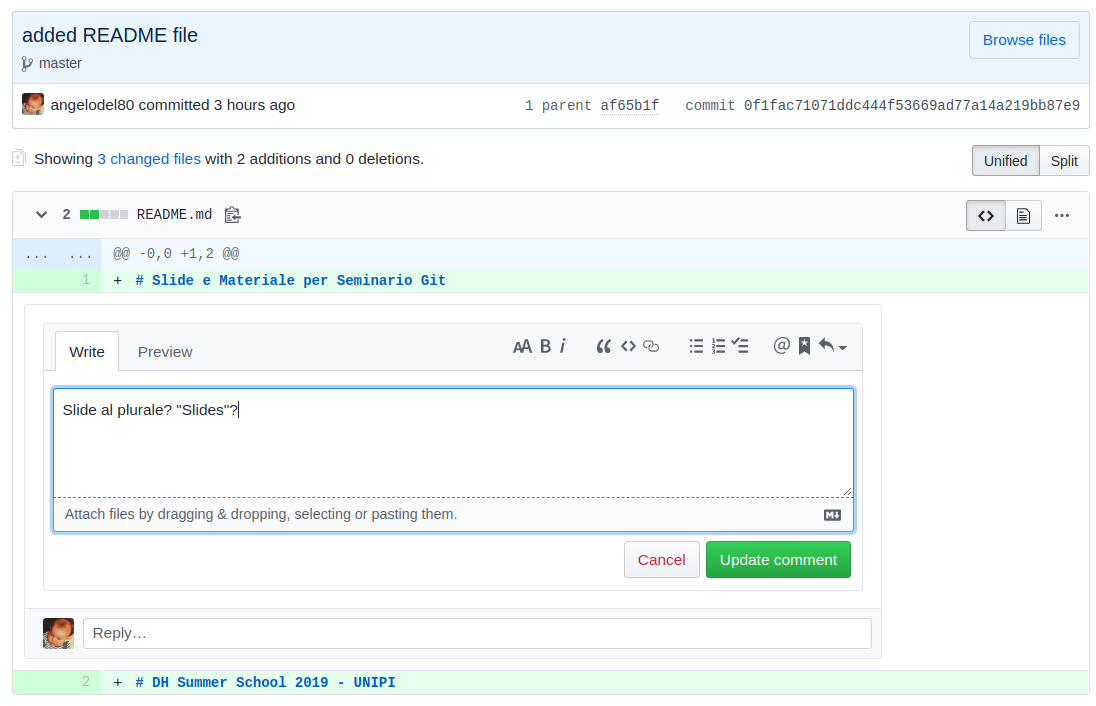
\includegraphics[width=.95\textwidth]{imgs/github-Commento-codice.png}
			\end{center}

\end{frame}

\begin{frame}
	\frametitle{Github}
	\framesubtitle{Comments to content lines}
	\addtocounter{nframe}{1}
	
		\begin{center}
			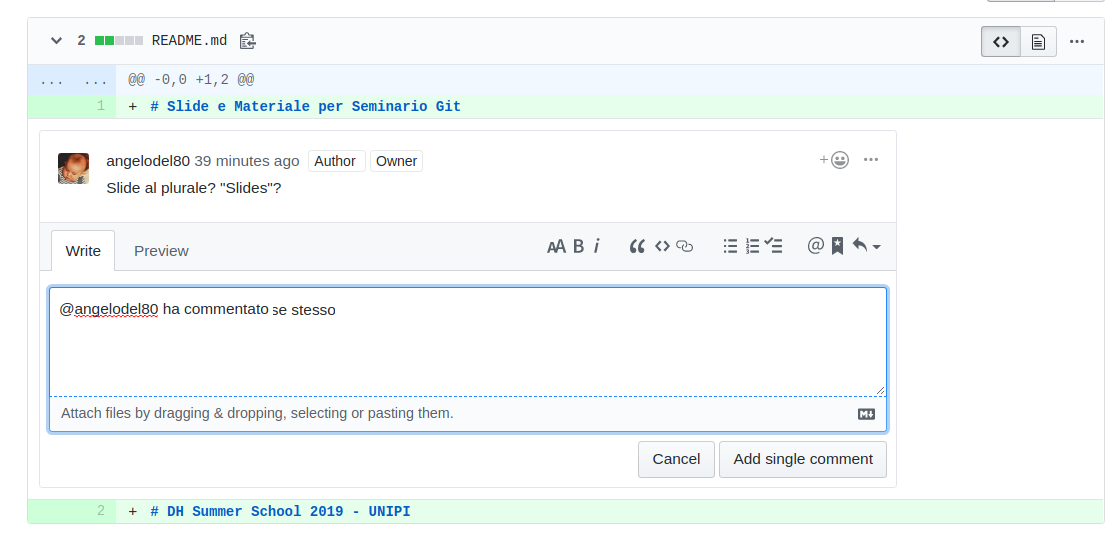
\includegraphics[width=.95\textwidth]{imgs/github-CommentoNotifica.png}
		\end{center}

\end{frame}
	

% \begin{frame}
% 	\frametitle{Rappresentazione digitale dei testi}
% 	\framesubtitle{basso e alto livello di codifica}
% 	\addtocounter{nframe}{1}

% 	\begin{block}{Codificare un testo}
% 		La codifica dei caratteri evidentemente non esaurisce i problemi per una opportuna rappresentazione delle caratteristiche interne ed esterne di un testo.
%     \end{block}
    
%     \begin{block}{Codificare un testo}
% 		Difatti la codifica del testo è una questione molto più complessa di una semplice riproduzione meccanica di un dato.
% 	\end{block}


% \end{frame}


% \begin{frame}
% 	\frametitle{Rappresentazione digitale dei testi}
% 	\framesubtitle{basso e alto livello di codifica}
% 	\addtocounter{nframe}{1}

% 	\begin{block}{Rappresentare un testo}
		
% 			La rappresentazione digitale di un testo è una operazione intrinsecamente assai difficile perché coinvolge una pletora di aspetti, a varie dimensioni, a varie granularità e a vari livelli di astrazione sia teorici, sia metodologici, sia tecnologici e sia pratici.
		
% 	\end{block}

% \end{frame}

% \begin{frame}
% 	\frametitle{Rappresentazione digitale dei testi}
% 	\framesubtitle{basso e alto livello di codifica}
% 	\addtocounter{nframe}{1}

% 	\begin{block}{Rappresentare un testo}
% 		\textbf{
% 			Prima di poter fare qualsiasi ipotesi su come compiere una codifica di un testo e su come rappresentarlo digitalmente, bisogna stabilire cosa si intende per testo.
% 		}
% 	\end{block}

% \end{frame}


% \begin{frame}
% 	\frametitle{Rappresentazione digitale dei testi}
% 	\framesubtitle{Modello dati di un testo}
% 	\addtocounter{nframe}{1}

% 	\begin{block}{Un testo non ha una struttura rigida, predefinita: }
% 		\begin{itemize}

% 			\item Non è rappresentabile solo come un insieme di record di un archivio elettronico.
% 			\item Non è rappresentabile solo come un insieme di tabelle di una banca dati.
% 			\item Non è rappresentabile solo come un albero o un insieme di sotto-alberi
% 			\item Non è rappresentabile solo come un grafo o come un insieme di sotto grafi

% 		\end{itemize}

% 	\end{block}

% \end{frame}

% \begin{frame}
% 	\frametitle{Molteplici modelli per diverse esigenze}
% 	\framesubtitle{Strutture dato e testo}
% 	\addtocounter{nframe}{1}

% 	\begin{block}{La rappresentazione di un testo}
% 		\begin{itemize}
% 			 %mia slide sulle possibili rappresentazioni del testo
% 			\item modello lineare: sequenza di dati non strutturati
% 			\item modello  a record: enumerazione delle proprietà
% 			\item modello tabulare: insieme di dati omogenei
% 			\item modello ad albero: gerarchie di dati e insiemi di dati
% 			\item modello grafo: rete di strutture informative interconnesse tra loro
%         \end{itemize}
        
% 	\end{block}
% \end{frame}



% \begin{frame}
% 	\frametitle{Elementi di Codifica del testo}
% 	\framesubtitle{Formalismi}
% 	\addtocounter{nframe}{1}

% 	\begin{block}{Formati di rappresentazione}
% 		\begin{center}
% 			Un formato è un insieme di regole e convenzioni formali per rappresentare un insieme di dati, nel nostro caso un testo.
% 		\end{center}

% 	\end{block}

% 	\begin{block}{Importanza dei formati}
% 		\begin{center}
% 			Seppur isomorfi la scelta dei formati condiziona molto l'efficienza delle operazioni e l'efficacia delle dichiarazioni.
% 		\end{center}

% 	\end{block}


% \end{frame}

% %\begin{frame}
% %    \frametitle{Elementi di Codifica del testo}
% %    \framesubtitle{lista di formati}
% %    \addtocounter{nframe}{1}
% %   
% %    \begin{block}{Formati dato}
% %Data structures – CSV and tabular data
% %– JSON
% %– RDF
% %Plain text formats – Plain text
% %– TeX, LaTeX, etc.
% %– Markdown, CommonMark and wiki syntaxes
% %Markup formats
% %– HTML, HTML5
% %– XML
% %– HTML5+ Embedded annotations (e.g., HTML5 + RDFa)
% %– Markup spinoffs for overlapping (e.g. LMNL, TexMECS, etc.) 
% %
% %    \end{block}

% % \begin{block}{Riferimenti TEI}
% %     Capitolo sul character encoding e modulo Ganji 
% % \end{block}

% %\end{frame}

% \begin{frame}
% 	\frametitle{Elementi di Codifica del testo}
% 	\framesubtitle{Tabella Formalismi}
% 	\addtocounter{nframe}{1}

% 	\begin{block}{Formalismi}
% 		\begin{center}
% 			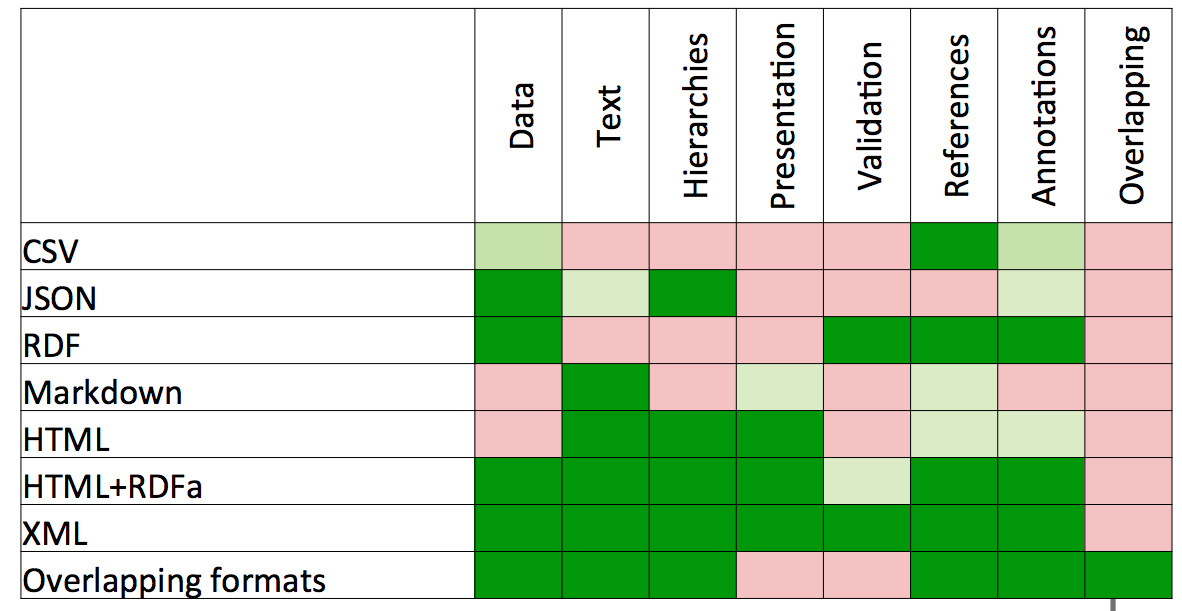
\includegraphics[width=.9\textwidth]{imgs/TabellaFormalismiCodificaTesto.png}
% 		\end{center}
% 	\end{block}
% 	courtesy of \textit{Fabio Vitali}

% \end{frame}


% \begin{frame}
% 	\frametitle{Elementi di Codifica del testo}
% 	\framesubtitle{Varietà di rappresentazione}
% 	\addtocounter{nframe}{1}

	
% 		\begin{center}
% 			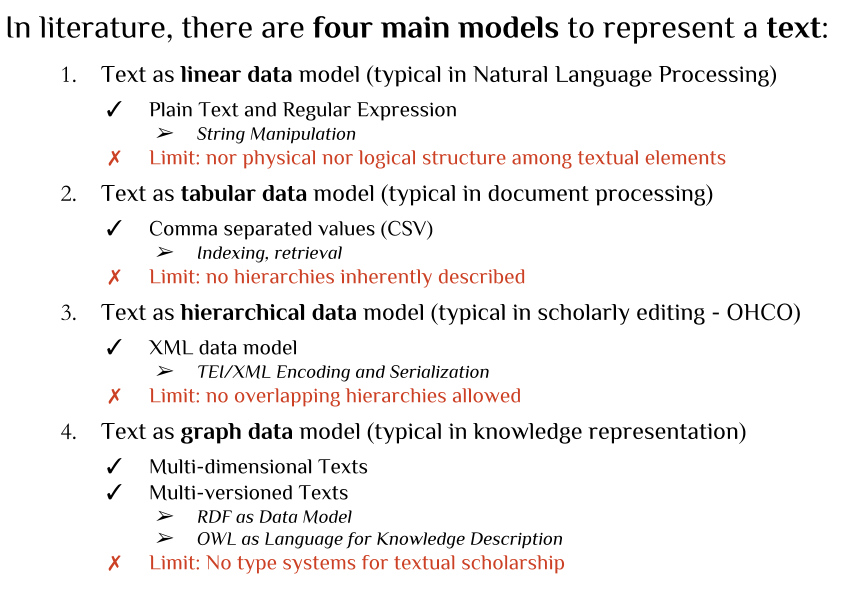
\includegraphics[width=.9\textwidth]{imgs/dataModels-slide.png}
% 		\end{center}
	
	
% \end{frame}

% \begin{frame}
% 	\frametitle{Elementi di Codifica del testo}
% 	\framesubtitle{Esempio di codifica del testo utilizzando CSV}
% 	\addtocounter{nframe}{1}

		
% 			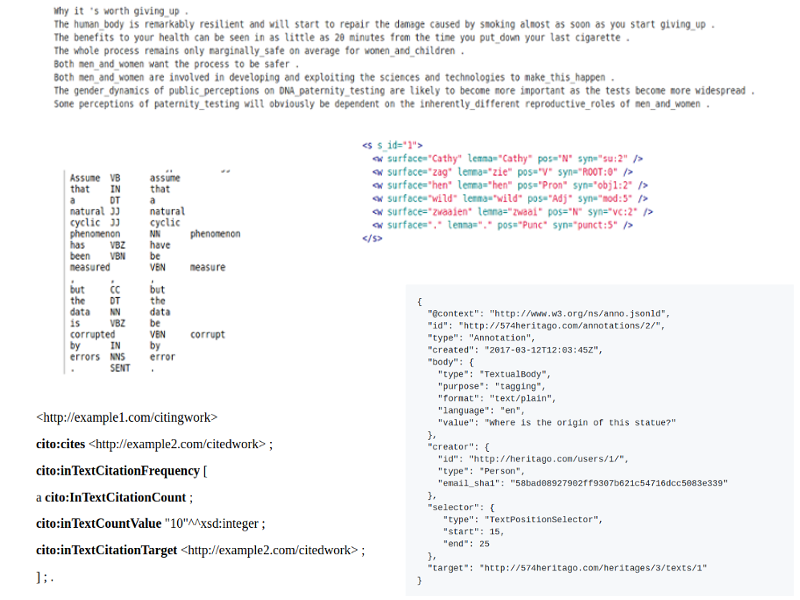
\includegraphics[width=1.1\textwidth]{imgs/VariRappresentazioniTesto.png}
		
	
% \end{frame}



% \begin{frame}
% 	\frametitle{Elementi di Codifica del testo}
% 	\framesubtitle{Formalismi}
% 	\addtocounter{nframe}{1}

% 	\begin{block}{Formati come formalismi}
% 		\begin{center}
% 			Data l'importanza metodologica il formato del dato diviene un vero e proprio formalismo, si parla cioè di linguaggi di codifica in quanto questi sistemi si basano su un insieme di istruzioni rigorose di codifica.
% 		\end{center}

% 	\end{block}

% \end{frame}



% \begin{frame}
% 	\frametitle{Elementi di Codifica del testo}
% 	\framesubtitle{Formalismi}
% 	\addtocounter{nframe}{1}

% 	\begin{block}{Formati e formalismi di codifica}

% 		Quindi ogni pezzo di informazione aggiunta ad un testo grezzo attraverso l'inserimento di dati metatestuali (markup, annotazione, codifica), constituisce il risultato di una analisi e di una interpretazione che è stata condotta (da un umano o da una macchina) al fine di esplicitare e rappresentare nel modo più accurato e completo possibile le informazioni da veicolare attraverso il formato digitale prescelto (anche in modo incrementale).


% 	\end{block}

% \end{frame}



 


 
% need to interact with GitHub at some point while using Git professionally

 
% This chapter is about using GitHub effectively.

 
% signing up for and managing an account

 
% creating and using Git repositories, common workflows to contribute to projects and to accept contributions to yours

 
% set up a free user account

 
% Sign up for GitHub

 
% GitHub will send you an email to verify the address you provided

 
% your dashboard page

 
% ready to use GitHub

 
% connect with Git repositories using the https:// protocol

 
% Next, if you wish, you can replace the avatar that is generated for you with an image of your choosing.

 
% people will see your avatar next to your username

 
% The way that GitHub maps your Git commits to your user is by email address

 
% extra security

 
% Two-factor Authentication

 
% Authentication is an authentication mechanism

 
% code in addition to your password whenever you log into GitHub.

 
% could be useful in helping you contribute to an existing project

 
% you don’t have push access, you can “fork” the project

 
% GitHub will make a copy of the project that is entirely yours

 
% it lives in your namespace, and you can push to it

 
% 170 about the change until the owner is happy with it

 
% In GitHub, a “fork” is simply the same project in your own namespace

 
% People can fork a project, push to it, and contribute their changes back to the original repository by creating what’s called a Pull Request

 
% This opens up a discussion thread with code review,

 
% the contributor can then communicate 170 about the change until the owner is happy with it

 
% at which point the owner can merge it in

 
% “Fork” button

 
% with your own writeable copy of the code.

 
% GitHub is designed around a particular collaboration workflow, centered on Pull Requests.

 
% teams use GitHub’s web based tools.

 
% Let’s walk through an example

 
% So let’s improve the program and submit it back to the project as a proposed change.

 
% we click the Fork button as mentioned earlier to get our own copy of the project.

 
% We will clone it locally, create a topic branch, make the code change and finally push that change back up to GitHub.

 
% git diff --word-diff

 
% [-delay(1000);-]{+delay(3000);+}

 
% [-delay(1000);-]{+delay(3000);+}

 
% Clone our fork of the project locally

 
% Create a descriptive topic branch

 
% Make our change to the code

 
% Check that the change is good

 
% Commit our change to the topic branch

 
% Push our new topic branch back up to our GitHub fork

 
% GitHub noticed that we pushed a new

 
% topic branch up and presents us with a big green button

 
% check out our changes and open a Pull Request to the original project

 
% give our Pull Request a title and description.

 
% unified diff of all the changes that will be made should this branch get merged by the project owner

 
% Create pull request button

 
% it’s also often used in internal projects at the beginning of the development cycle

 
% the project owner can look at the suggested change and merge it

 
% reject it or comment on it

 
% on GitHub this happens online

 
% leave a comment by clicking on any of the lines

 
% Anyone can also leave general comments on the Pull Request.

 
% both commenting on a line of code

 
% leaving a general comment in the discussion section

 
% with GitHub you simply commit to the topic branch again and push, which will automatically update the Pull Request

 
% Adding commits to an existing Pull Request doesn’t trigger a notification

 
% This button only shows up if you have write access to the repository and a trivial merge is possible

 
% If you click it GitHub will perform a “non-fast-forward” merge, meaning that even if the merge could be a fast-forward, it will still create a merge commit.

 
% This is the basic workflow that most GitHub projects use

 
% Topic branches are created, Pull Requests are opened on them, a discussion ensues, possibly more work is done on the branch and eventually the request is either closed or merged.

 
% initiate the code review and discussion process

 
% No forking necessary

 
% creating, maintaining and administering your own project.

 
% Let’s create a new repository to share our project code with

 
% All you really have to do here is provide a project name;

 
% click the “Create Repository” button

 
% new repository on GitHub,

 
% Since you have no code there yet, GitHub will show you instructions for how to create a brand-new Git repository, or connect an existing Git project.

 
% Now that your project is hosted on GitHub, you can give the URL to anyone you want to share your project with.

 
% It is often preferable to share the HTTPS based URL for a public project

 
% The HTTPS one is also exactly the same URL they would paste into a browser to view the project there.

 
% If you’re working with other people who you want to give commit access to, you need to add them as “collaborators”

 
% you want to give them push access to your repository, you can add them to your project.

 
% “push” access

 
% both read and write access to the project and Git repository

 
% Then select “Collaborators”

 
% You can repeat this as many times as you like to grant access to everyone you like

 
% revoke access, just click the “X”

 
% get a Pull Request yourself.

 
% Pull Requests can either come from a branch in a fork of your repository or they can come from another branch in the same repository.

 
% The only difference is that the ones in a fork are often from people where you can’t push to their branch and they can’t push to yours,

 
% with internal Pull Requests generally both parties can access the branch.

 
% The other interesting URLs are the .diff and .patch URLs, which as you may guess, provide unified diff and patch versions of the Pull Request.

 
% As we covered in The GitHub Flow, you can now have a conversation with the person who opened the Pull Request.

 
% comment on specific lines of code

 
% Once the code is in a place you like and want to merge it in, you can either pull the code down and merge it locally, either with the git pull <url> <branch> syntax we saw earlier, or by adding the fork as a remote and fetching and merging.

 
% If you decide you don’t want to merge it, you can also just close the Pull Request and the person who opened it will be notified.

 
% neat trick tha

 
% If you see a Pull Request that is moving in the right direction and you have an idea for a change that depends on it or you’re not sure is a good idea, or you just don’t have push access to the target branch, you can open a Pull Request directly to it.

 
% Mentions and Notifications

 
% GitHub also has a pretty nice notifications system

 
% In any comment you can start typing a @ character and it will begin to autocomplete with the names and usernames of people who are collaborators or contributors in the project.

 
% pulling people into conversations rather than making them poll

 
% You will also be subscribed to something if you opened it, if you’re watching the repository or if you comment on something

 
% no longer wish to receive notifications, there is an “Unsubscribe” button

 
% If you go to the “Notification center” tab from the settings page, you can see some of the options you have.

 
% The two choices are to get notifications over “Email” and over “Web” and you can choose either,

 
% Web notifications only exist on GitHub and you can only check them on GitHub

 
% If you click on that, you will see a list of all the items you have been notified about

 
% Email notifications are the other way you can handle notifications through GitHub

 
% It’s also worth noting that if you have both email and web notifications enabled and you read the email version of the notification, the web version will be marked as read as well if you have images allowed in your mail client.

 
% There are a couple of special files that GitHub will notice if they are present in your repository.

 
% The first is the README file, which can be of nearly any format that GitHub recognizes as prose. For example, it could be README, README.md, README.asciidoc, etc. If GitHub sees a README file in your source, it will render it on the landing page of the project.

 
% Many teams use this file to hold all the relevant project information for someone who might be new to the repository or project. This generally includes things like:

 
% What the project is for

 
% How to configure and install it

 
% An example of how to use it or get it running

 
% The license that the project is offered under

 
% How to contribute to it

 
% Since GitHub will render this file, you can embed images or links in it for added ease of understanding.

 
% Generally there are not a lot of administrative things you can do with a single project, but there are a couple of items that might be of interest.

 
% If you would like to transfer a project to another user or an organization in GitHub, there is a “Transfer ownership” option at the bottom of the same “Options” tab of your repository settings page that allows you to do this.

 
% This is helpful if you are abandoning a project and someone wants to take it over

 
% move it into an organization.

 
% sets up a redirect from your URL

 
% In addition to single-user accounts, GitHub has what are called Organizations

 
% Organizational accounts have a namespace where all their projects exist

 
% These accounts represent a group of people with shared ownership of projects

 
% many tools to manage subgroups of those people

 
% companies

 
% New organization” from the menu

 
% First you’ll need to name your organization and provide an email address for a main point of contact for the group

 
% When you create new repositories you can create them either under your personal account or under any of the organizations that you are an owner in

 
% Organizations are associated with individual people by way of teams

 
% grouping of individual user accounts and repositories within the organization

 
% Teams make this easy, without having to manage the collaborators for every individual repository.

 
% ou can use to add members to the team

 
% Each team can have read only, read/write or administrative access to the repositorie

 
% “Settings” button

 
% Additionally, team @mentions (such as @acmecorp/frontend) work much the same as they do with individual users, except that all members of the team are then subscribed to the thread

 
% Organizations also give owners access to all the information about what went on under the organization. You can go to the Audit Log tab and see what events have happened at an organization level, who did them and where in the world they were done.

 
% curl

 
% GitHub user

 
% how to create an account

 
% manage an organization,

 
% create and push to repositories

 
% contribute to other people’s projects

 
% ccept contributions from others

 
% ource code control

 
% basic tasks of tracking and committing files

 
% important actions occur